
\documentclass[preprint,12pt]{elsarticle}

\usepackage[spanish]{babel}
\usepackage{amssymb}
\usepackage{graphicx}
\usepackage{lineno}
\usepackage[utf8]{inputenc}
\usepackage{url}
\usepackage{color}
\usepackage{enumerate} 
\usepackage[hidelinks]{hyperref}


\begin{document}
	
	\begin{frontmatter}
		
		
		\title{\huge DataWarehouse vs  Datalake}
		
		\author{Mamani Ayala, Brandon        (2015052715)}
		\author{Quispe Mamani, Angelo	      (2015052826)}
		\author{Vizcarra Llanque, Jhordy	      (2015052719)}
		\author{Ordoñez Quilli, Ronald          (2015052821)}
		\author{Rodriguez Mamani, Juan      (2017057862)}
		
		\address{Tacna, Perú}
		
		\begin{abstract}
			%% Text of we
			
The data warehouses in English take each importance day, as organizations move from schemes of only data collection to schemes of analysis of the same. However, in spite of the great diffusion of the concepts related to data warehouses, there is not too much Information available in Spanish regarding the methodologies fo implement them In this short article we will try to provide a general explanation of one of the most used methodologies. 
		\end{abstract}
\end{frontmatter}
%%

	
	%%
	%\linenumbers
	
	%% main text
	\section{Resumen}
Los almacenes de datos (data warehouses en inglés) toman cada día mayor importancia, a medida que las organizaciones pasan de esquemas de sólo recolección de datos a esquemas de análisis de los mismos. Sin embargo a pesar de la gran difusión de los conceptos relacionados con los almacenes de datos, no existe demasiada información disponible en castellano en cuanto a las metodologías para implementarlos. En este breve artículo intentaremos brindar una explicación general de una de las metodologías más usadas \\
	%%
	
	%%
	%\linenumbers
	
	%% main text



	%%
	
	%%
	%\linenumbers
	
	%% main text
\section{Introduccion}
\section{DataWarehouse}

Definición de Bill Inmon\\
\\Fue uno de los primeros autores en escribir sobre el tema de los almacenes de datos, define un data warehouse (almacén de datos) en términos de las características del repositorio de datos:

\begin{itemize}
	\item Orientado a temas: Los datos en la base de datos están organizados de manera que todos los elementos de datos relativos al mismo evento u objeto del mundo real queden unidos entre sí.
	\item Variante en el tiempo: Los cambios producidos en los datos a lo largo del tiempo quedan registrados para que los informes que se puedan generar reflejen esas variaciones.
	\item No volátil: La información no se modifica ni se elimina, una vez almacenado un dato, éste se convierte en información de sólo lectura, y se mantiene para futuras consultas.
	\item Integrado: La base de datos contiene los datos de todos los sistemas operacionales de la organización, y dichos datos deben ser consistentes.
\end{itemize}

Definición de Ralph Kimball\\
\\Define un almacén de datos como: "Es un almacén de datos que extrae, limpia, conforma y entrega una fuente de datos dimensional para la consulta y el análisis". También fue Kimball quien determinó que un data warehouse no era más que: "la unión de todos los Data marts de una entidad". Defiende por tanto una metodología ascendente (bottom-up) a la hora de diseñar un almacén de datos.


\subsection{Materiales y Metodos}

ESTRUCTURA\\
\\La arquitectura de un data warehouse puede ser dividida en tres estructuras simplificadas: básica, básica con un área de ensayo y básica con área de ensayo y data marts.

\begin{itemize}
	\item Con una estructura básica, sistemas operativos y archivos planos proporcionan datos en bruto que se almacenan junto con metadatos. Los usuarios finales pueden acceder a ellos para su análisis, generación de informes y minería.
	\item Al añadir un área de ensayo que se puede colocar entre las fuentes de datos y el almacén, ésta proporciona un lugar donde los datos se pueden limpiar antes de entrar en el almacén. Es posible personalizar la arquitectura del almacén para diferentes grupos dentro de la organización.
	\item Se puede hacer agregando data marts, que son sistemas diseñados para una línea de negocio en particular. Se pueden tener data marts separados para ventas, inventario y compras, por ejemplo, y los usuarios finales pueden acceder a datos de uno o de todos los data marts del departamento.
\end{itemize}

\begin{center}
	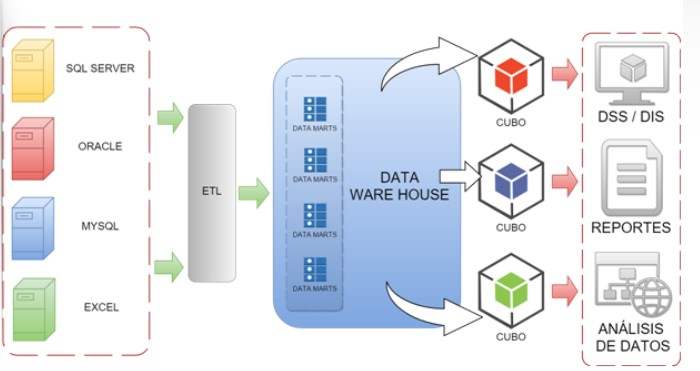
\includegraphics[width=12cm]{./Imagenes/imagen1} 
\end{center}

ETL (Extract-Transform-Load)\\
\begin{itemize}
	\item Extracción: obtención de información de las distintas fuentes tanto internas como externas.
	\item Transformación: filtrado, limpieza, depuración, homogenización y depuración de la información.

\begin{center}
	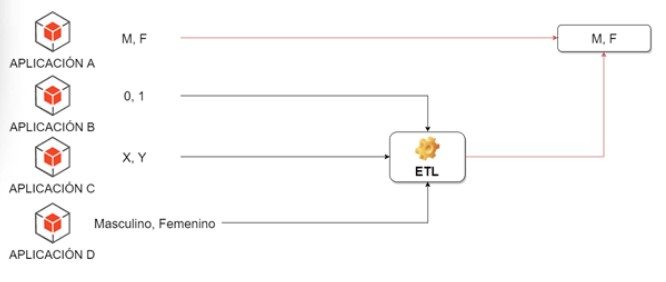
\includegraphics[width=12cm]{./Imagenes/imagen2} 
\end{center}

	\item Carga: Organización y actualización de los datos y los metadatos de la base de datos.
\end{itemize}

DATA MART\\
\\Es una base de datos departamental, especializada en un área de negocio especifica. Se caracteriza por disponer la estructura optima de datos para analizar el informacional detalle desde todas las perspectivas que afecten a los procesos de dicho negocio.

\begin{center}
	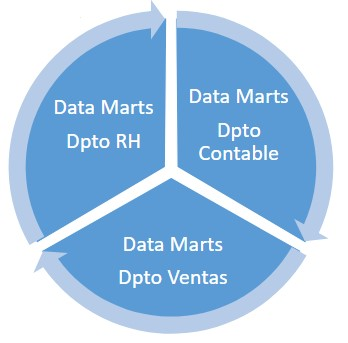
\includegraphics[width=6cm]{./Imagenes/imagen3} 
\end{center}

CUBOS\\
\\Es una base de datos especial, en la cual el almacenamiento físico de los datos se realiza en un vector multidimensional.
\begin{center}
	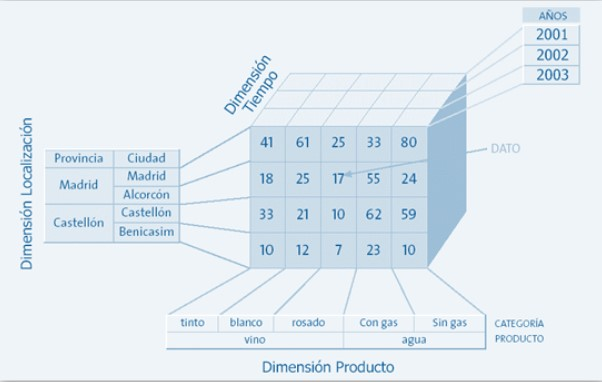
\includegraphics[width=12cm]{./Imagenes/imagen4} 
\end{center}

Diferencias con un DB Transaccional\\
\begin{center}
	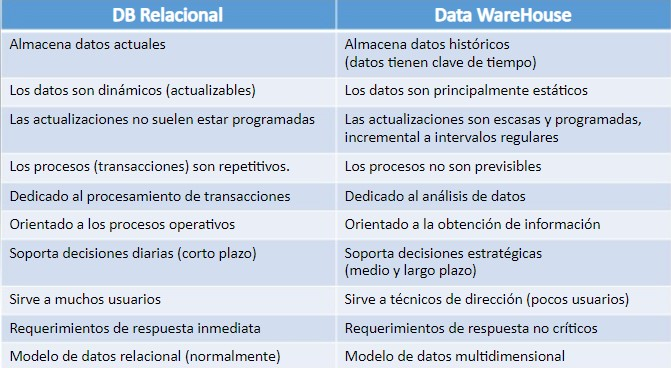
\includegraphics[width=12cm]{./Imagenes/imagen5} 
\end{center}

HERRAMIENTAS\\
\begin{center}
	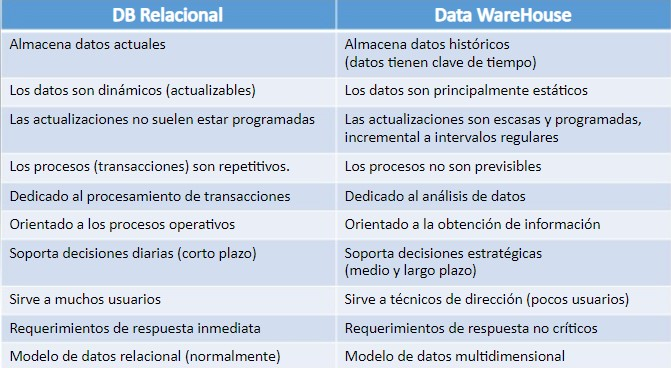
\includegraphics[width=12cm]{./Imagenes/imagen5} 
\end{center}

\subsection{Resultados}

\subsection{Conclusiones}

\begin{itemize}
	\item Las particiones no se procesaban en paralelo si no secuencialmente, lo que hace que sea más lento el procesamiento.
	\item No se pueden usar multiples idiomas.
	\item Si son muchos datos tarda bastante en manejar configuraciones de diferentes particiones.
	\item El modelo tabular acapara demasiada memoria RAM y a su vez es dependiente de tal que afectará a otras aplicaciones.
\end{itemize}

\section{Datalake}

\subsection{Materiales y Metodos}

\subsection{Resultados}

\subsection{Conclusiones}

\begin{itemize}
	\item Las particiones no se procesaban en paralelo si no secuencialmente, lo que hace que sea más lento el procesamiento.
	\item No se pueden usar multiples idiomas.
	\item Si son muchos datos tarda bastante en manejar configuraciones de diferentes particiones.
	\item El modelo tabular acapara demasiada memoria RAM y a su vez es dependiente de tal que afectará a otras aplicaciones.
\end{itemize}



%%
	
	%%
	%\linenumbers
	
	%% main text

	
	\newpage
	
		%ESTILO
	%ARCHIVO .bib
	   \begin{thebibliography}{0}
              \bibitem{Juan} https://bib.irb.hr/datoteka/102195.t09r02.pdf 
                 \bibitem{Juan} https://www.sarjen.com/2016/03/15/what-are-the-pros-and-cons-of-tabular-model-over-multi-dimension-cube-and-relation-database/
                 \bibitem{Juan} https://www.element61.be/en/resource/choice-between-tabular-or-multidimensional-models-sql-server-analysis-services-2012
                  \bibitem{Jhordy} https://docs.microsoft.com/es-es/sql/analysis-services/comparing-tabular-and-multidimensional-solutions-ssas?view=sql-server-2017
 \bibitem{Jhordy} https://www.businessintelligence.info/definiciones/que-es-modelo-dimensional.html
                    \bibitem{Brandon} https://www.businessintelligence.info/definiciones/que-es-modelo-dimensional.html


         \end{thebibliography}
	
\end{document}

%%
%% End of file `elsarticle-template-1-num.tex'.
